% \documentclass[format=acmtog]{acmart}    
% \documentclass{acmart}    
\documentclass[acmtog, authorversion]{acmart}

\usepackage{booktabs} % For formal tables
\usepackage[ruled]{algorithm2e} % For algorithms
\renewcommand{\algorithmcfname}{ALGORITHM}
\SetAlFnt{\small}
\SetAlCapFnt{\small}
\SetAlCapNameFnt{\small}
\SetAlCapHSkip{0pt}
\IncMargin{-\parindent}

\usepackage[latin1]{inputenc}
\usepackage{graphicx}
\usepackage{amsmath}
\usepackage{amsfonts}

% Metadata Information
% \acmJournal{PACMHCI}
\acmVolume{9}
\acmNumber{4}
\acmArticle{39}
\acmYear{2010}
\acmMonth{3}
\acmArticleSeq{11}

\setcopyright{usgovmixed}

% \acmDOI{0000001.0000001}

% Paper history
\received{February 2007}
\received{March 2009}
\received[accepted]{June 2009}

\DeclareMathOperator*{\argmax}{argmax}

\begin{document}

\title{Researcher name extraction from faculty directories}

\author{Jo�o Mateus de Freitas Veneroso}
% \affiliation{%
%   \institution{Universidade Federal de Minas Gerais}
%   \streetaddress{Av. Pres. Ant�nio Carlos, 6627 - Pampulha}
%   \city{Belo Horizonte}
%   \state{MG}
%   \postcode{31270-901}
%   \country{Brazil}}
\email{jmfveneroso@gmail.com}

\begin{abstract}

Public databases such as DBLP and Google Scholar contain valuable information 
about the academic environment that have been incredibly useful
helping answering numerous research questions. However, in these databases, only 
a fraction of the records contain researcher affiliation information, and even 
in the cases where the information is present it is frequently outdated. The 
problem can be better or worse depending on the field of study.
We propose a method to extract researcher names from faculty directories
automatically in order to keep up to date information about researcher 
affiliation and be general enough to solve any name extraction task.
Various web data extraction methods have already been proposed in
the literature and they typically lack either in generality, because
wrappers trained on a set of examples do not perform well when handling
different websites, or precision, because domain agnostic methods
perform poorly compared to domain specific methods.
Our statistical NLP approach solves the name extraction task with 
a framework that incorporates both textual and structural features to
yield an excellent tradeoff between generality and precision. 
We conducted experiments over a collection of 310 faculty 
web pages from multiple universities across the world and obtained 94.37\%
precision, 97.61\% recall and 0.9596 F-measure.


\end{abstract}

\keywords{Information extraction, statistical classifier, natural language processing}

\maketitle

% ==========================================
% Beginning of text.                       |
% ==========================================

\section{Introduction}

Web data extraction is the task of automatically extracting structured information
from unstructured or semi-structured web documents. Tipically, Information Extraction 
tasks consist of mapping unstructured or poorly
structured data to a semantically well defined structure. The input is most commonly
composed of a set of documents that describe a group of entities in a similar manner,
while the Information Extraction task deals with identifying those entities and 
organizing them according to a template. 

HTML documents most often lie in between the structured / unstructured data paradigm, which means that 
authors take a rather relaxed approach in regard to formal structure. Hierarchy, element disposition,
class names, and other features related to the document structure and indirectly associated
with the data itself are valuable information in the task of identifying entities and 
determining relationships, yet we cannot expect these features to be completely constrained by 
any underlying pattern. Like natural language, organization patterns tend to follow some guidelines 
but are in no way subject to strict rules.

We are interested in the task of name extraction, particularly extracting researcher names from 
university websites to complement data from public databases such as the DBLP repository 
(http://dblp.uni-trier.de/) in order to allow broad international research group comparison 
and enquiring about publication patterns. The DBLP database has sparse information about author 
affiliation and only contains information about computer science researchers. With our 
probabilistic method we hope to build a general approach to solve this problem without having
to rely on metadata from PDF papers and handle the name extraction problem in general.

\begin{figure}
  \centering
  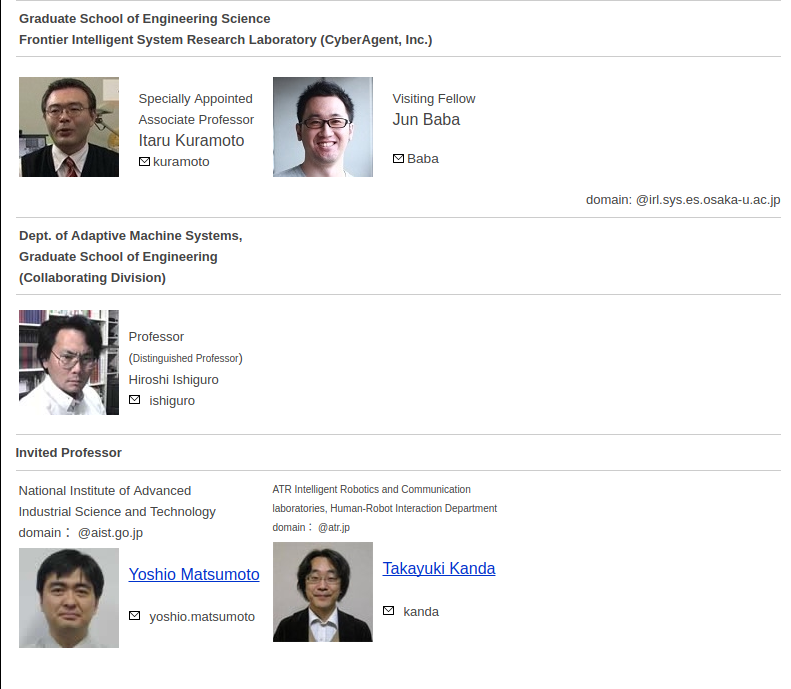
\includegraphics[width=0.5\textwidth]{pics/jap_intelligent_robotics_lab}
  \caption{Example of a faculty directory}
  \label{fig:faculty_directory}.
\end{figure}

In order to acknowledge the complexity of this extraction task take for example a snippet of 
the staff page for the intelligent robotics laboratory from Osaka University shown in figure 
\ref{fig:faculty_directory}. There is some structure to the way member profiles are arranged, 
but the organization is rather flexible even considering this single website. Other websites 
can show very different patterns, ranging from tables and lists to free form.

Researcher names can happen inside plain text, similar to typical named entity recognition 
scenarios. Names may be part of larger sentences such as in "Michael Johnson Chair" and "John 
Doe Avenue" yielding false positives. Names can be composed of common words (e.g. Summer Hall) 
yielding false negatives. In short, there is no one rule that fits all cases.

State-of-the-art named entity recognition approaches such as Conditional Random Fields do not 
perform so well in information extraction cases such as the one presented in figure 
\ref{fig:faculty_directory}, because the text is insufficient to provide any contextual information 
about the semantic category of a word. 

Since we lack a database with all possible name combinations, we propose a 
hollistic statistical method that accounts for discrepancies in data organization by assigning 
probabilities to sequences of tokens without relying on per-website training. Our method of
label assignement resembles a Naive Bayesian classifier without the assumption of 
token independence. We also rely as little as possible on contextual information to avoid
the mistakes of other classifiers. The base model already achieves recall and precision rates 
above 90\%, but the performance can be increased even further by incorporating HTML structural
features to estimate better probabilities, specially to avoid filtering out false negatives.


\section{Related Work}

In the last 20 years, the astonishing growth of public information in the web has 
led to the development of a number of different approaches to the problem of web 
data extraction. Traditionally, the task was solved by designing special purpose
programs called wrappers to recognize relevant data and store it in a structured
format. These early tools varied wildly relative to their degree of automation. 

It was readily perceived that manual wrapper generation was a rather tedious and
error prone process, unsuited for large scale operations. Wrappers tend to
break frequently because they rely heavily on web page features that can change 
often. So, in the late nineties, several authors advocated for wrapper induction, a technique 
that consists of automatically constructing wrappers from a small set of examples by 
identifying delimiters or context tokens that single out the desired attributes. 
Some remarkable wrapper induction methods are WIEN \cite{Kushmerick2000}, Soft 
Mealy \cite{Hsu1998} and STALKER \cite{Muslea1999}.

Despite being better than constructing wrappers manually, wrapper induction methods 
still suffered from a lack of expressive power and flexibility. These methods had 
trouble handling records with missing attributes or unusual structures because
patterns could only be identified if they happened at least once in the examples.

Other approaches such as NoDoSE (\cite{Adelberg1998}) and Debye (\cite{Laender2002a}) 
brought greater flexibility to wrapper induction methods by requiring a greater level 
of human interaction through graphical user interfaces. Web data extraction techniques often 
require some sort of assistance from human experts to boost accuracy. One of the main challenges 
in the field lies in determining an adequate tradeoff between the degree of automation and 
the precision and recall of the data extraction tool.

In order to automate the task of web data extraction completely some approaches,
such as Road Runner \cite{Crescenzi2001}, removed entirely the need for data examples.
Road Runner parses documents belonging to a same class (e.g. books on Amazon) and 
generated wrappers based on their similarities and differences, yielding comparable results 
to those obtained by wrapper induction methods. However like previous approaches, it was 
unsuited for cross site extraction tasks because the learned rules weren't general enough.

NLP based approaches aimed at extracting more general rules that could possibly
be employed over multiple websites. RAPIER \cite{Califf1999} is a method of rule
extraction that uses information such as part-of-speech tags and semantic classes from
a lexicon to derive patterns from a set of training examples. This approach is more
flexible than the wrapper induction methods, however it achieves much lower rates of 
recall and precision.

In 2002, a survey by Laender et al. \cite{Laender2002} made a thorough classification of the
early approaches with a taxonomy based on their main technology, being them: languages for
wrapper development, HTML-aware tools, NLP-based tools, Wrapper Induction Tools,
Modeling-based tools and Ontology-based tools. Some noteworthy examples from this era
are: 

\begin{itemize}
\item TSIMMIS \cite{Hammer1997} and WebOQL \cite{Arocena1999}, which are special purpose 
languages for building wrappers.

\item Road Runner \cite{Crescenzi2001}, XWRAP \cite{Liu2000} and W4F \cite{Sahuguet1999}, 
which are HTML-aware tools that infer meaningful patterns from the HTML structure.

\item RAPIER \cite{Califf1999}, SRV \cite{Freitag1998}, WHISK \cite{Soderland1999}, which 
are NLP-based tools.

\item WIEN \cite{Kushmerick2000}, Soft Mealy \cite{Hsu1998} and STALKER \cite{Muslea1999} which 
are wrapper induction methods.

\item NoDoSE \cite{Adelberg1998} and Debye \cite{Laender2002a}, which are semi supervised modeling
based tools that require some interaction with the user by means of a graphical
user interface.
\end{itemize}

In 2006, Chang et. al. \cite{Chang2006} complemented the previous surveys with semisupervised 
technologies such as Thresher \cite{Hogue2005}, IEPAD \cite{Chang2001} and 
OLERA \cite{Chang2004}. They differed from supervised 
and unsupervised methods because they either needed only a rough description of
data from users for extraction rule generation or some level of post processing
that needed user attention. The survey also mentioned newer unsupervised methods
such as DeLa \cite{Wang2003}, Exalg \cite{Arasu2003} and Depta \cite{Zhai2005}.

Most of the early information extraction systems were rule-based with either 
manual rule description or automatic rule learning from examples, thus they
suffered from a lack of flexibility when dealing with noisy and unstructured data.
Huge progress in the field of statistical learning led to the development of
statistical models that tried to solve this problem.

In 2008, Sarawagi \cite{Sarawagi2008} produced a survey that classified wrappers in
rule-based methods, statistical methods and hybrid models, bringing together
the fields of named entity recognition, relationship extraction and information
extraction. The rule based methods encompass most of the previous models. The statistical 
methods convert the extraction task into a token labeling task, identifying the 
target entities through the assignment of labels.
Any classifiers such as a Support Vector Machines, Logistic Classifiers or
Neural Networks could be employed to perform this task. However Hidden Markov Models, 
Maximum Entropy Taggers and Conditional Random Fields tend to perform better at most
extraction tasks because of the way they model token and label dependencies. Hybrid models
incorporate both rule-based and statistical methods.

Statistical models have proven to be reliable tools for performing numerous NLP tasks. 
However, information from web documents relevant to data extraction tasks is usually 
arranged in a tabular form rather than in a plain text format. Therefore, typical state
of the art classifiers can yield poor results if they rely exclusively on textual 
information. In the web information extraction task, the document structure must be 
incorporated as a feature in an effective classifier.

More recently, surveys by \cite{Ferrara2014} and \cite{Schulz2016} updated the 
previous surveys with some interesting innovations. Some examples are: the Visual 
Box Model \cite{Krupl2005}, a data extraction system that produces a visualization of 
the web page to exploit visual cues to identify data presented in a tabular form;
automatic wrapper adaptation \cite{Ferrara2011}, a tecnique that tries to reduce the cost of 
wrapper maintenance by measuring the similarity of HTML trees and adapting
wrappers to the new page structure; AutoRM \cite{Shi2015}, a method to mine
records from a single web page by identifying similar data regions through DOM
tree analysis; and Knowledge Vault \cite{Dong2014}, a method that combines different 
extraction approaches to feed a probabilistic knowledge base.

In 2016, Varlamov et. al. \cite{Varlamov2016} argued that the degree of automation can no
longer be the main classification criterion for the data extraction systems
because unsupervised methods which were widely considered to be the state 
of the art when dealing with individual websites performed poorly or were
innapropriate on cross site extraction tasks. The authors proposed a 
classification of methods by the extent of their application. 
The competing approaches were separated into two groups: methods for individual 
websites and methods that are applicable to whole application domains. 

The first group contains most of the earlier approaches, including the supervised
approaches: SRV (\cite{Freitag1998}), RAPIER (\cite{Califf1999}), WHISK (\cite{Soderland1999}), 
WIEN (\cite{Kushmerick2000}) SoftMealy (\cite{Hsu1998}) and STALKER (\cite{Muslea1999}); and
the unsupervised approaches: RoadRunner (\cite{Crescenzi2001}) and EXALG (\cite{Arasu2003}).

The second group is divided between domain specific methods and domain agnostic methods.
Domain specific methods are designed for extracting data about a particular 
application domain across multiple websites.
Domain specific methods integrate information about the particular application domain in the 
course of its development and thus are able to achieve superior performance in
comparison to domain agnostic methods.
One example is the method of comment extraction 
from blog posts described by Kao et. al. \cite{Kao2010}. By incorporating multiple tecniques and 
domain specific features they are able to build a classifier that differentiates comment-blocks 
and non-comment blocks. This is only one of many methods tuned for various domains.
Our name extractor method also belongs to this category. 

Domain agnostic methods are the most general extraction methods. They can extract
information from any application domain from multiple websites. They pose the hardest
challenge because the tool must infer data relevance without any prior training in
that particular application domain. Some examples are: ODE (\cite{Su2009}), ObjectRunner 
(\cite{Abdessalem2010}), and AMBER (\cite{Furche2012}). These approaches are broader but 
yield worse results than domain specific methods.


\section{Implementation Overview}

The name extraction problem is no different from a Named Entity Recognition problem, however 
approaches that tipically achieve high accuracy on NER tasks like Conditional Random Fields, 
Hidden Markov Models or Maximum Entropy Models do not necessarily perform so well when
handling tabular data, as is most common in web data extraction tasks. For example, in 
narrative text, a classifier could learn patterns such as "X spoke to Y" and then discover from 
the sentence "Alice spoke to Bob" that Alice and Bob are names. However in the name extraction task,
the lack of context words prevents these methods from detecting useful patterns over sequences 
of tokens. We are also interested in developing a method to extract researcher names regardless of 
the website's main language, even though at this moment we won't be considering non extended-ASCII 
encodings such as chinese and farsi characters. Training classifiers over multiple corpuses in 
different languages could be in itself a very challenging task. Instead we rely on a priori 
probabilities and structural HTML features to attribute label probabilities to tokens. When manually 
scanning through faculty pages in search of researcher names, the intuitive method to extract them 
is usually identifying a few cases that we are sure are researcher names (e.g. Dr. John Smith),
then identifying structural patterns to classify other cases for which we may be not so sure, 
either because they lie outside our knowledge base (e.g. T.J. Shi) or because they sound like
common words (e.g. Summer Hall).


\subsection{Pre-processing}

Before applying the classifier over the web page content, we must run the input target
through a series of pre-processing steps in order to clean the data as much as possible.
The HTML document is first parsed producing a DOM tree. At this stage, malformed HTML is
converted into a valid DOM tree as it is commonly done in most browsers nowadays. Header 
details, script tags, style tags, hidden tags and comments are removed. Spaces, tabs, 
newlines and special characters are as used as separators in a tokenization stage producing 
a list of tokens. Each token is saved as an object with the following attributes:

\begin{description}
\item [Value:] the token's text in lowercase with converted accented characters.
\item [DOM Element:] a pointer to the DOM Element that contains this token in the DOM Tree.
\item [Previous Token:] the previous token object.
\item [Next Token:] the next token object.
\end{description}

With this simple structure we can extract all kinds of features, with the benefit of 
having a list of tokens such as the one we would obtain from a plain text format. Through
the DOM Element pointer we can figure out the parent elements, nesting depth, siblings and other
useful information that can be used to improve estimations.


\subsection{Name Extraction}

Let $ t = (t_1, t_2, ..., t_n) $ be a sequence of token objects obtained on the pre-processing
stage, and $ y = (y_1, y_2, ..., y_n) $ be a sequence of labels attributed to these tokens
where $ y_i $ can be either a "Name Label" (N), meaning that token $ t_i $ is a person's name, or
a "Word Label" (W), meaning that token $ t_i $ is a common word (not a person's name). Then,
the problem of extracting names from a sequence of tokens is just a series of binary classification 
problems. Considering that each token $ t_i $ has a probability $ P(t_i = y_i) $ of having label 
$ y_i $, the problem of finding an optimal sequence of labels $ y^* $ for a sequence of tokens 
$ t $ can be written as:

\begin{equation}
\\
y^* = \argmax_y P(t_1 = y_1, t_2 = y_2, ..., t_n = y_n)\\
\\
\label{eq:1}
\end{equation}

We may employ the chain rule to explore the relationship between joint and conditional 
probabilities. For ease of exposure, consider that $ P(Y_i) \equiv P(t_i=y_i) $ yielding:

\begin{equation}
\\
P(Y_1, Y_2, ..., Y_n) = P(Y_1) P(Y_2|Y_1) ... P(Y_n|Y_{n-1}, Y_{n-2}, ...)
\\
\label{eq:2}
\end{equation}

A k-gram model could approximate the probabilities $ P(Y_1, Y_2, ..., Y_n) $ by looking
only to the first $ k $ tokens and sliding a window of a fixed size $ k $ over the token
sequence. However, the conditional probabilities $ P(Y_i|Y_{i-1}, ...) $ are hard to
estimate, because the joint distribution $ P(Y_i) \equiv P(t_i=y_i) \equiv P(t_i, y_i) $
depends both on the previous labels and the previous tokens. If we express them 
in terms of joint probabilities the problem becomes more evident:

\begin{equation}
\\
P(Y_i|Y_{i-1}, Y_{i-2}, ...) \equiv P(t_i, y_i|t_{i-1}, y_{i-1}, t_{i-2}, y_{i-2}, ...)
\\
\label{eq:3}
\end{equation}

So we make the assumption that the probability that token $ t_i $ has label $ y_i $ depends
on the values of previous labels but is independent of the previous tokens. For example, 
given a sequence of tokens $ \{"John", "Smith"\} $, the conditional probability $ P("Smith"|"John"=Name) $ 
is equivalent to $ P("Smith"|Any\ name) $. In other words, this means that the probability of 
Smith being a last name is the same regardless of a person's first name, as long as we can make sure 
that the previous token is a name. Equation \ref{eq:3} then becomes:

\begin{equation}
\\
P(Y_i|Y_{i-1}, Y_{i-2}, ...) = P(t_i, y_i|y_{i-1}, y_{i-2}, ...)
\\
\label{eq:4}
\end{equation}

Once again we can employ the chain rule to obtain:

\begin{equation}
\\
P(t_i, y_i|y_1, y_2, \ldots, y_{i-1}) = P(t_i|y_i, y_{i-1}, ...)P(y_i|y_{i-1}, y_{i-2}, ...) \\
\\
\label{eq:5}
\end{equation}

In equation \ref{eq:5}, the probability $ P(t_i|y_i, y_{i-1}, ...) $ depends on the current and
previous labels. We make a simplifying assumption that $ P(t_i|y_i, y_{i-1}, ...) $ can
be approximated by $ P(t_i|y_i) $. The reasoning behind it is that previous labels have
neglible influence over the value of token $ t_i $. For example, we assume that $ P(t_i="John"|t_i=Name) $ 
is a good aproximation for $ P(t_i="John"|t_i=Name, t_{i-1}=Word, ...) $. With this assumption, 
equation \ref{eq:5} becomes: 

\begin{equation}
\\
P(t_i, y_i|y_1, y_2, \ldots, y_{i-1}) = P(t_i|y_i)P(y_i|y_{i-1}, y_{i-2}, ...) \\
\\
\label{eq:6}
\end{equation}

Finally, by replacing equation \ref{eq:6} in equation \ref{eq:2} and grouping together
the second terms of equation \ref{eq:6} to form the joint probability 
$ P(y_1, y_2, \ldots, y_n) $, equation \ref{eq:2} becomes:

\begin{equation}
\\
P(Y_1, Y_2, \ldots, Y_n) = P(y_1, y_2, \ldots, y_n) P(t_1|y_1)P(t_2|y_2) \ldots P(t_n|y_n) 
\label{eq:7}
\end{equation}

Equation \ref{eq:7} can be split into two parts: the prior, given by the first part of the 
equation on the right side and the conditional token probabilities, given by the rest of the 
equation on the right side.


\subsubsection{Prior probabilities}

The prior probabilities are given by the expression $ P(y_1, y_2, \ldots, y_n) $, which
represent the probability of a series of tokens assuming labels $ \{ y_1, y_2, ..., y_n \} $
without any prior knowledge about the actual token values.

By assuming a window of size $ k \leq n $ we may approximate the priors by calculating the
joint probability $ P(y_1, y_2, \ldots, y_k) $. In this case we need to acquire estimates for 
all possible sequences of labels. Considering that label $ y_i $ must be either a name or a word,
then there are $ 2^k $ different combinations for a window of size $ k $.

Let $ N $ be a name label and $ W $ be a word label, then for a window of size $ k $ we 
would need to estimate prior probabilities for all $ 2^k $ possible sequences of labels.
In practice, a window of size $ 4 $ seems to be accurate enough. In this case, the
sequences would be: $ \{W, W, W, W\}, \{W, W, W, N\}, \{W, W, N, W\}, \ldots $.

When names occur next to each other we have no way to tell where the first name ends and 
the second one starts. In order to delimit name boundaries we need to estimate
priors for different sequences of name labels in addition to our previous priors.
Let the first and second name labels be $ N_1 $ and $ N_2 $, respectively. Then,
we need to estimate priors for the sequences: $ \{W, N_1, N_1, N_2\} $, 
$ \{W, N_1, N_1, N_2\} $, $\{W, N_1, N_2, N_2\} $, $ \ldots $. In practice, we are never interested
in isolated occurrences of name labels so we can exclude combinations such as
$ \{W_1, N_1, N_2, N_2\} $.

Most of the times when names happen inside a list they tend to be contained inside a 
single HTML element. 
Eventhough this is not always the case, this knowledge can be incorporated as an
additional piece of evidence in our model. This evidence becomes specially useful 
when we are trying to delimit name boundaries. Let $ * $ indicate a breaking point in 
a sequence of labels, so $ {W, W*,N, N} $ means that the tokens taking labels WW
are contained inside a single HTML element, while the remaining tokens are inside 
different HTML elements.
We could estimate sequences with multiple breaking points, however a single breaking
point has shown good results. For our window of size 4, we need to estimate all prior 
probabilities with the 4 possible breaking points:
$ \{y_1, y_2, y_3, y_4\} $, $ \{y_1*, y_2, y_3, y_4\} $, $ \{y_1,y_2*, y_3, y_4\} $, $ \{y_1, y_2, y_3*,y_4\} $.


\subsubsection{Conditional token probabilities}

We need to estimate conditional token probabilities for both labels: names and words.
So we need to know $ P(t_i|N) $, the probability that a name is $ t_i $ and
$ P(t_i|W) $, the probability that a word is $ t_i $.

For our experiments, the conditional token probabilities were obtained by maximum
likelihood estimation with Laplace smoothing to account for tokens that
didn't occur in the corpus. The $ P(t_i|N) $ probabilities were estimated over a 
collection of approximately 1.5 million names from the DBLP database. The
$ P(t_i|W) $ probabilities were estimated over a corpus of 100 thousand documents
obtained during the crawling stage. In the latter case all capitalized words 
were ignored when estimating probabilities in order to remove most names
from the corpus.

Token probabilities can be made more precise by incorporating features
in equation \ref{eq:7}. We do that by changing the token conditional 
probabilities to:

\begin{equation}
\\
P(t_i, f_1, f_2, \ldots, f_n|y_i) = P(t_i|y_i)P(f_1|y_i) \ldots P(f_n|y_i)
\\
\label{eq:8}
\end{equation}

where $ f_i $ are features, which are assumed to be independent between themselves.
The features can be textual or structural. Textual features take textual
clues like previous words and token length to predict if a given token is a name.
Structural features infer token probabilities based on the HTML structure
like tag names and nesting depth. In practice previous and 
next words weren't particularly effective in empirical tests, possibly due
to the fact that most names occured in lists in the test collection. So they were
removed from the features list.

Structural features estimated over the entire corpus end up being too general
so they help little in increasing token probability estimates. HTML structure 
varies radically between different documents such that the only stable characteristic 
is that names tend to have similar structural contexts in the same faculty
directory. For example, if all names appear inside a <tr> tag in a given document 
it does not mean that names tend to appear inside <tr> rather than any other tag
in other documents. However for that particular document we may be able to identify 
other names and exclude words by knowing that tokens occuring inside <tr> tags
have a higher probability of being names.

If our basic algorithm (without structural features) was able to extract a
good number of names from a page on the first passing, we may use
their structural context to estimate probabilities for our structural 
features. Of course those tokens that were tagged as words can be used
to estimate the word conditional probabilities. On a second passing we can
incorporate these improved estimates to boost the model's precision 
considerably. This process can be repeated multiple times to further 
increase peformance.

\begin{table}[h]
  \small
  \begin{center}
    \begin{tabular}{ |l|l|l| }
      \hline
      Id & Feature & Description \\
      \hline
      1  & Token incidence      & How often a token happens in a document         \\
      2  & Token length         & The token's character length                    \\
      3  & First+Second parents & First and second HTML parents combined          \\
      4  & Third parent         & Third HTML parent                               \\
      5  & CSS class name       & Innermost CSS class valid for the token         \\
      6  & Child number         & The child number relative to the HTML parent    \\
      7  & Nesting depth        & The number of HTML parents up to root           \\
      \hline
    \end{tabular}
  \end{center}
  \caption{Features}
  \label{tab:features}
\end{table}

Table \ref{tab:features} describes the features tested in our experiments. A couple of
other features were tested, but they weren't included in the analysis due to the lack
of significant impact on the results. Some of them were: next word
indicates some location (street, avenue, etc.), previous word is an honorific, 
token is capitalized, token is the first child in an HTML element, etc. 


\subsection{Experiments}

\begin{table}[h]
  \begin{center}
    \begin{tabular}{ |l|l|l|l| }
      \hline
      Features & Precision & Recall & F-measure \\
      \hline
      None  & 91.71\% -        & 91.39\% -        & 0.9155          \\ 
      1     & 91.28\% (0.3880) & 93.79\% (0.1836) & 0.9252 (0.3026) \\ 
      2     & 92.00\% (0.4189) & 92.03\% (0.4086) & 0.9201 (0.4042) \\
      1+2   & 91.83\% (0.4660) & 93.90\% (0.1586) & 0.9285 (0.2336) \\
      \hline
    \end{tabular}
  \end{center}
  \caption{Textual features experiment}
  \label{tab:base_model}
\end{table}


The test collection was a set of 310 manually labeled faculty directory pages. 
For each model the precision, recall and f-measures were calculated. All
measures were tested for statistical significance with a one tailed paired T-test, the 
t-values are presented inside parenthesis next to each measure. Results were
considered to be significant when the t-value was smaller than 0.05.

Extracted names were only considered to be correct 
when they resulted on an exact match with the test data. All measures were obtained by the averaged 
results of a 5 fold cross validation run. We first compared the textual features on our base 
model (NE), which passes only one time over the token list. The results are presented in table 
\ref{tab:base_model}. 

\begin{table}[h]
  \begin{center}
    \begin{tabular}{ |l|l|l|l| }
      \hline
      Features & Precision & Recall & F-measure \\
      \hline
      3         & 93.43\% (0.1280) & \textbf{96.14\% (0.361)} & 0.9477 (0.475)           \\
      4         & 93.04\% (0.1965) & 95.67\% (0.508) & 0.9433 (0.740)                    \\
      5         & 93.04\% (0.1781) & 95.50\% (0.653) & 0.9425 (0.819)                    \\
      6         & 92.70\% (0.2307) & \textbf{95.60\% (0.451)} & 0.9413 (0.725)           \\
      7         & 92.83\% (0.2374) & \textbf{95.79\% (0.467)} & 0.9429 (0.789)           \\
      3 + 5 + 7 & 94.23\% (0.0664) & \textbf{97.14\% (0.163)} & \textbf{0.9566 (0.212)}  \\
      \hline
    \end{tabular}
  \end{center}
  \caption{Structural features experiment}
  \label{tab:ne_2}
\end{table}

Next, we tested the structural features in a model that passes two times over the 
token list, estimating the structural feature probabilities on the second passing. 
We used the best set of textual features found in the previous experiment. The results 
are presented in table \ref{tab:ne_2}.

\begin{table}[h]
  \begin{center}
    \begin{tabular}{ |l|l|l|l| }
      \hline
      \# passings & Precision & Recall & F-measure \\
      \hline
      2 & 94.40\% (0.525) & \textbf{97.48\% (0.117)} & \textbf{0.9592 (0.151)} \\ 
      3 & 94.37\% (0.544) & \textbf{97.58\% (0.104)} & \textbf{0.9595 (0.141)} \\
      4 & 94.40\% (0.523) & \textbf{97.61\% (0.100)} & \textbf{0.9597 (0.135)} \\
      5 & 94.37\% (0.544) & \textbf{97.61\% (0.100)} & \textbf{0.9596 (0.138)} \\
      \hline
    \end{tabular}
  \end{center}
  \caption{Multiple passings experiment}
  \label{tab:ne_plus}
\end{table}

Finally we compared models with 1, 2, 3, 4 and 5 passings over the token list using the 
best set of features from the previous experiments. The results are presented on 
table \ref{tab:ne_plus}.

By comparing the results, it becomes clear that incorporating structural features
with the two passing strategy improved all metrics significantly, even though the
precision improvements came slightly above our significance threshold. By design, the
features were chosen with improvements to recall rather than precision in mind. Because
when a data extractor misses useful results, it becomes hard to obtain that data, 
however cleaning bad results is a much simpler task to be carried manually.


\subsection{Further Research}

Our model is finely tuned for the particular problem of researcher name extraction, 
but we believe this result can be generalized to solve other data extraction 
problems. Furthermore, the researcher affiliation data collected by the name extractor 
still needs to be used for evaluating the reputation metric proposed by \cite{Ribas2015}
in the research group classification task.

% ==========================================
% End of text.                             |
% ==========================================

\nocite{*}
\bibliographystyle{unsrt}
\bibliography{bibfile}

\end{document}
